\documentclass[english,a4]{article}

%\usepackage{fontspec}
\usepackage{amsmath,amsthm,amssymb}
%\usepackage{unicode-math}
%\usepackage{polyglossia}
\usepackage{enumitem}
\usepackage{tikz,tikz-cd}
\usepackage{hyperref}
\usepackage{microtype}
%\usepackage[explicit]{titlesec}
\usepackage[mathscr]{euscript}
\usepackage{mathtools}

\input macros%
\input macros2%

\hypersetup{
    colorlinks,
    linkcolor={red!50!black},
    citecolor={blue!50!black},
    urlcolor={blue!80!black}
}

\setlist[enumerate]{label=(\roman*)}

\title{{On Symmetries of Spheres in HoTT-UF}}%
\author{\normalsize XYZ} %
\date{\normalsize Last updated on \today}%

%% global tikz styles
\tikzset{cell/.style={%
    shorten <=1em,%
    shorten >=1em,
    /tikz/commutative diagrams/Rightarrow
  }%
}%

\def\U{\universe U}%

\begin{document}

\maketitle

\begin{abstract}
  We first prove in HoTT-UF that
  \begin{displaymath}
    (\Sc = \Sc) \weq (\Sc + \Sc).
  \end{displaymath}
This result doesn't generalise to higher dimensions.
However, one can prove that $S^n = S^n$ is equivalent the sum of two
connected components, since the set truncation of $S^n = S^n$ is $\bool$. 
One component contains, of course, $\refl{S^n}$.
The other component contains ...
Moreover, these two components are equivalent.
\end{abstract}


\section{The circle}
In this document, we shall establish an equivalence
between the type of equalities of $\Sc$ with itself and the sum type
of $\Sc$ with itself. We work in intuitionistic Martin-Löf's type
theory with $\Sigma$-, $\Pi$- and $\mathrm{Id}$- types and with a
cumulative hierarchy of universes, simply written $\U$, for
which Voevodsky's univalence axiom hold. Moreover we introduce the
circle as a higher inductive type, meaning we postulate the existence
of a type $\Sc$ together with terms:
\begin{align}
  \label{eq:1}
  \base &: \Sc\\
  \Sloop &: \base =_{\Sc} \base
\end{align}
This type enjoys a inductive property: given a type family
$T : \Sc \to \U$, an element $t:T(\base)$ and a path
$p:t=_{T(\base)}t$, the $\Sc$-induction property provides a dependent
function $f : \prod_{x:\Sc}T(x)$ such that $f(\base) \jdeq t$ and an
element $q: f(\Sloop) = p$. In particular, $\Sc$-induction provides a
map
\begin{equation}
  \label{eq:2}
  \left(\sum_{t:T(\base)} \pathover t T \Sloop t\right) \to \prod_{x:\Sc}T(x)
\end{equation}
that is easily shown to be an equivalence (through $\Sc$-induction
again). In the case $T$ is the family constant in $A:\U$, it gives the
following universal property of the circle:
\begin{equation}
  \label{eq:3}
  \left(\sum_{t:A}t=t\right) \weq \left( \Sc \to A \right)
\end{equation}

Using univalence, one gets that $(\Sc = \Sc)$ is
equivalent to $(\Sc \weq \Sc)$ and we shall then concentrate on
proving
\begin{equation}
  (\Sc \weq \Sc) \weq (\Sc+\Sc)
\end{equation}
As usual, we shall denote $f:\Sc\weq\Sc$ for a map $f:\Sc\to \Sc $
such that the proposition $\isEq(f)$ is non-empty instead of the more
honest $(f,!):\Sc \weq \Sc$. 
This is harmless as the first projection is an equivalence
\begin{equation}
  ((f,!) =_{\Sc \weq \Sc} (g,!)) \simeq (f=_{\Sc \to \Sc}g).
\end{equation}

Recall that for each $x:\Sc$ one has an equivalence:
\begin{equation}
  \label{eq:8}
  f_x : (\base = \base) \to (x=x)
\end{equation}
Indeed, such a map $x\mapsto f_x$ is defined by $\Sc$-induction by
setting $f_{\base} \defequi \id$ and $f_{\Sloop}$ to be the proof that
postcomposing with the conjugation $\Sloop \blank \inv\Sloop$ is the
identity. In particular one can easily prove that
$f_x(\Sloop^k) = f_x(\Sloop)^k$ for any $k:\zet$. Now define $\iota_1$
and $\iota_2$ on each $x:\Sc$ as follows:
\begin{align*}
  \iota_1(x) (\base) &\defequi x & \iota_2(x) (\base) &\defequi x,
  \\
  \iota_1(x)(\Sloop) &\defis f_x(\Sloop) &  \iota_2(x)(\Sloop) &\defis f_x(\Sloop)^{-1}
\end{align*}
Each $\iota_j(x)$ ($j\in\{1,2\}$) is indeed an equivalence: $\Sc$
being connected, the proposition $\isEq(\iota_j(x))$ has to be proved
for only one point, say $\base$; but $\iota_1(\base)$ is equal to
$\id_\Sc$ (hence an equivalence) and $\iota_2(\base)$, that we call
$-\id_\Sc$ in the following, is its own pseudo inverse.

The maps $\iota_1$ and $\iota_2$ induce a maps
$\iota \defequi \langle\iota_1,\iota_2\rangle : \Sc + \Sc \to (\Sc\weq
\Sc)$.
\begin{theorem*}
  The map $\iota$ is an equivalence.
\end{theorem*}
%
Before proving the theorem, here is a lemma that already explains that
the two components of $\Sc+\Sc$ are mapped to distinct parts of
$(\Sc \weq \Sc)$.
\begin{lemma}
  \label{lemma:id-not-equal-oppid}%
  The type $(\id_\Sc = -\id_\Sc)$ is empty.
\end{lemma}
\begin{proof}
  By function extensionality and $\Sc$-induction, an element
  $p : \id_\Sc = -\id_\Sc$ is given by the data of
  $p(\base) : \id_\Sc(\base) = -\id_\Sc(base)$, that is
  $p(\base):\base=\base$, together with a pathover
  $p(\Sloop): \pathover {p(\base)} {} \Sloop {p(\base)}$ in the type
  family $x\mapsto \id_\Sc (x)=-\id_\Sc (x)$. The transport over
  $\Sloop$ in this type family is given by
  $\inv\Sloop\blank\inv\Sloop$, so that $p(\Sloop)$ is equivalently
  given by an element of $\inv\Sloop p(\base) \inv\Sloop =
  p(\base)$. By expliciting $p(\base)$ as $\Sloop^k$ for some
  $k:\zet$, the last equation becomes
  $\inv \Sloop \Sloop^k \inv \Sloop = \Sloop^k$, leading to the
  contradiction $2=0$ in $\zet$.
\end{proof}

\begin{proof}[Proof of the theorem]
  Take an element $\phi : \Sc \weq \Sc$ and consider the fiber of
  $\iota$ at $\phi$:
  \begin{equation}
    \label{eq:fiber-iota-two-components}%
    \inv\iota(\phi) \jdeq \sum_{x:\Sc+\Sc} \phi = \iota(x)
    \weq \left(\sum_{x:\Sc}\phi = \iota_1(x)\right) +
    \left(\sum_{x:\Sc}\phi = \iota_2(x)\right)
  \end{equation}
  One wants to prove the proposition $\iscontr(\inv\iota(\phi))$,
  hence one may assume a path $q:\phi(\base) = \base$ instead of
  merely $\Trunc{\phi(\base) = \base}$. By the description of the
  symmetries of $\base:\Sc$, there is $k:\zet$ such that
  $q\phi(\Sloop)\inv q = \Sloop^k$. Denoting $\psi$ for a pseudo
  inverse of the equivalence $\phi$, one also gets
  $q':\psi(\base) = \base$ and subsequently $\ell:\zet$ such that
  $q'\psi(\Sloop)\inv{q'} = \Sloop^\ell$. Doing some path algebra it
  follows that:
  \begin{equation}
    \label{eq:4}
    \psi(\phi(\Sloop)) = \inv{(q' \psi(q))}\Sloop^{\ell k} (q' \psi(q))
  \end{equation}
  By hypothesis, one has also $\tau : \prod_{x:\Sc}\psi\phi(x) = x$,
  so there is a pathover of type
  $\pathover {\tau(\base)} {} \Sloop {\tau(\base)}$ in the type family
  $x \mapsto \psi(\phi(x)) = x$. The transport over $\Sloop$ in this
  family is given by $\Sloop \blank \inv{(\psi\phi(\Sloop))}$, so that
  \begin{equation}
    \label{eq:5}
    \Sloop \tau(\base) \inv{(\psi\phi(\Sloop))} = \tau(\base)
  \end{equation}
  Putting equations~(\ref{eq:5}) and~(\ref{eq:4}) together, one find
  \begin{equation}
    \label{eq:6}
    \inv{(q' \psi(q) \inv{\tau(\base)})} \Sloop^{\ell k} (q' \psi(q) \inv{\tau(\base)}) = \Sloop
  \end{equation}
  However, conjugation in $\base = \base$ is equal to the identity, so
  that in the end $\Sloop^{\ell k} = \Sloop$, or otherwise put
  $\ell k = 1$ in $\zet$. Using the decidability of equality on
  $\zet$, one can show that the only invertible elements of $\zet$ are
  $1$ and $-1$. So $k = 1$ or $k = -1$. We proceed by case:
  \begin{enumerate}
  \item If $k=1$, then $Q \defequi (q, !)$ is element of
    $\phi = \id_\Sc$, where the term $!$ of the proposition
    $q=\Sloop q \inv{\phi(\Sloop)}$ is given by path algebra from the
    hypothesis $q\phi(\Sloop)\inv q=\Sloop^k$ ($k$ being $1$ here). We
    can then only show $\iscontr(\inv\iota(\id_\Sc))$ to conclude (by
    transport over $\inv Q$) that $\iscontr(\inv\iota(\phi))$. 

    One can immediately see that the second component of the right
    hand-side in equation~(\ref{eq:fiber-iota-two-components}) is
    empty when instantiated with $\id_\Sc$ for $\phi$: indeed,
    $\false$ being a proposition and $\Sc$ being connected, one only
    need to check that $\id_\Sc = \iota_2(\base)$ is contradictory;
    and because $\iota_2(\base) \jdeq -\id_\Sc$, it follows from
    lemma~\ref{lemma:id-not-equal-oppid}.

    Hence it remains to prove that $\sum_{x:\Sc}\id_\Sc=\iota_1(x)$ is
    contractible. For $x:\Sc$, the type $\id_\Sc = \iota_1(x)$ is
    equivalent (through first function extensionality and then
    $\Sc$-induction) to
    $\sum_{p:\base=\iota_1(x)(\base)}\pathover p T \Sloop p$ where $T$
    is the type family $y\mapsto y=\iota_1(x)(y)$. Now
    $\iota_1(x)(\base)\jdeq x$ and the transport over the loop
    $\Sloop$ in the type family $T$ is given by
    $\iota_1(x)(\Sloop) \blank \inv \Sloop$. In other words,
    \begin{equation}
      \label{eq:10}
      (\id_\Sc = \iota_1(x)) \weq \sum_{p:\base = x}f_x(\Sloop)p = p {\Sloop}
    \end{equation}
    By induction on $p:\base=x$, one can see that the proposition
    $f_x(\Sloop)p=p\Sloop$ is always satisfied. In the end, one has
    \begin{equation}
      \label{eq:11}
      \left(\sum_{x:\Sc}\id_\Sc=\iota_1(x)\right)
      \weq
      \left(\sum_{x:\Sc}\base=x\right)
    \end{equation}
    The type on the right is a singleton, hence contractible. This
    concludes the case $k=1$.
      \item The case $k=-1$ is completely similar to the case $k=1$. We
    now have a proof that $\phi = -\id_\Sc$, hence we shall prove that
    $\iscontr(\inv\iota(-\id_\Sc))$. From there one can determine that
    the first component of in (\ref{eq:fiber-iota-two-components}) is
    empty and concentrate on proving that
    $\sum_{x:\Sc}-\id_\Sc = \iota_2(x)$. The type
    $-\id_\Sc = \iota_2(x)$ is equivalent to
    $\sum_{p:\base = x}\inv{f_x(\Sloop)}p=p\inv\Sloop$ which is again
    equivalent to $\base=x$. We conclude the proof in the same way by
    recognizing a singleton.
  \end{enumerate}
\end{proof}

\section{The sphere}
\newcommand{\Sp}{S^2}%
\newcommand{\mrd}{\mathit{merid}}%
\newcommand{\susp}[1]{\operatorname{\Sigma}{#1}}%
\newcommand{\Truncset}[1]{\Trunc{#1}_0}%
\newcommand{\truncset}[1]{\trunc{#1}_0}%
\newcommand{\Truncprop}[1]{\Trunc{#1}}%
\newcommand{\truncprop}[1]{\trunc{#1}}%
\newcommand{\ptdto}{\to_\ast}%
\newcommand{\flip}{\operatorname{flip}}%
\newcommand{\conncomp}[2]{{#1}_{(#2)}}%
%
We define the sphere $\Sp$ as the suspension $\susp\Sc$ of the circle.
The suspension $\susp A$ of a type $A$ is a higher inductive type 
with two point constructors and path constructors indexed by $A$:
\begin{align}
  \label{eq:suspension}
  N &: \susp A \quad\text{the `North pole'}\\
  S &: \susp A \quad\text{the `South pole'}\\
  \mrd &: A \to (N =_{\susp A} S) \quad\text{the `meridians'}
\end{align}
Suspensions enjoy a inductive property: given a type family
$T : \susp A \to \U$, elements $n:T(N)$ and $s:T(S)$, and paths
$m(a) : n=_{\mrd(a)}s$ for all $a:A$, 
suspension induction provides a dependent
function $f : \prod_{x:\susp A}T(x)$ such that $f(N) \jdeq n$, $f(S) \jdeq s$,
and paths $p_f(a): f(\mrd(a)) = m(a)$ for all $a:A$.

\subsection{Roadmap}
\label{sec:roadmap}

For the sphere $\Sp$, topological intuitions make very unlikely to
construct a proof of $(\Sp + \Sp) \weq (\Sp = \Sp)$. We shall target a
lesser goal: prove that $(\Sp = \Sp)$ has two equivalent connected
components, and investigate some of the elements of both these
components. Through univalence, it is enough to do so for the type
$(\Sp \weq \Sp)$. The first step is to provide a dependent function
\begin{equation}
  \label{eq:14}
  \prod_{f:\Sp \weq \Sp} \Truncprop{e_0=f} + \Truncprop{e_1=f}
\end{equation}
where $e_0$ and $e_1$ are two equivalences to be defined afterwards
that embody the role of $\id_\Sc$ and $-\id_\Sc$ in the case of
$\Sc$. One of the key property is that $e_0 \neq e_1$, so that for
each $f: \Sp \weq \Sp$, the type
$P(f) \defequi \Truncprop{e_0=f} + \Truncprop{e_1=f}$ is a
proposition. Hence, for a given $f$, in proving $P(f)$ one might as
well suppose a path $f_0: N = f(N)$ instead of the mere fact that
$\Truncprop{N=f(N)}$. In other words, one can suppose that $f$ is a
pointed equivalence. We shall show how to produce a map\footnote{This
  map is {\tt \color{red} (should be)} related to the usual degree of
  pointed endomaps of $\Sp$ as follows: for $f:\Sp \ptdto \Sp$, under
  the equivalence $\pi_2(\Sp) \weq \zet \weq (\base = \base)$, the
  induced group morphism $\pi_2(f)$ identifies with $\ap{\phi(f)}$.}
\begin{equation}
  \label{eq:18}
  \phi: (\Sp \ptdto \Sp) \to (\Sc \to \Sc)
\end{equation}
such that $\phi(\id_{\Sp},\refl N) = \id_\Sc$ and such that
$\phi(g\circ f) = \phi(g) \circ \phi(f)$. (In other words, $\phi$ is a
morphism of monoids.) In particular $\phi$ sends pointed equivalences
to equivalences $\Sc \weq \Sc$, which we already know to be merely
equal either to $\id_\Sc$ or $-\id_\Sc$. From the definition of $e_0$
and $e_1$, it will be obvious that $\phi(e_0) = \id_\Sc$ and
$\phi(e_1) = -\id_\Sc$. The proposition (\ref{eq:14}) will be
eventually proved once it is shown that
$\Truncprop{\phi(f) = \phi(g)} \implies \Truncprop{f=g}$.

The second step is to prove that the component
$\sum_{f:\Sp \weq \Sp}\Truncprop{e_0=f}$ is equivalent to
$\sum_{f:\Sp \weq \Sp}\Truncprop{e_1=f}$. For that purpose, we shall
construct a map $\flip : (\Sp \to \Sp) \to (\Sp \Sp)$ where $\flip(f)$
is defined by induction as follows:
\begin{equation}
  \label{eq:19}
  \begin{aligned}
    \flip(f)(N) &\defequi f(N)
    \\
    \flip(f)(S) &\defequi f(S)
    \\
    \flip(f)(\mrd(\base)) &\defis f(\mrd(\base))
    \\
    \flip(f)(\mrd(\Sloop)) &\defis \inv{f(\mrd(\Sloop))}
  \end{aligned}
\end{equation}
This is an equivalence, as it is its own pseudoinverse. In addition,
it is easily seen that $\flip(e_0) = \flip(e_1)$. Hence, $\flip$ is an
equivalence that sends the connected component at $e_0$ into the
connected component at $e_1$. The equivalence from
$\conncomp{(\Sp\weq\Sp)}{e_0}$ to $\conncomp{(\Sp\weq\Sp)}{e_1}$ is
obtained by restraining $\flip$ to $\conncomp{(\Sp\weq\Sp)}{e_0}$, and
co-restraining it to $\conncomp{(\Sp\weq\Sp)}{e_1}$.

\subsection{Degree}
\label{sec:winding-numbers}
\def\hopffam{\mathcal H}%
\def\loopspace#1{\operatorname{\Omega_{#1}}}%

In associating a degree in $\ZZ$ to very pointed map $\Sp \to \Sp$,
the first step is usually to define a map
$\loopspace 2 \Sp \to \loopspace 1 \Sc$. The construction of such a
map in HoTT is known material that can be tracked back at least to
Brunerie's thesis. It goes through the construction of a
type-theoretical version of the Hopf fibration that we shall follow
carefully.

Consider the type family $\hopffam : \Sp \to \U$ defined by induction
as follows:
\begin{equation}
  \label{eq:7}
  \begin{aligned}
    \hopffam (N) &\defequi \Sc
    \\
    \hopffam (S) &\defequi \Sc
    \\
    \hopffam (\mrd(x)) &\defis \iota_1(x) \quad\text{defined above}
  \end{aligned}
\end{equation}
Denote $X$ for the total space of the type family $\hopffam$. One can
show that $X$ is equivalent to the 3-sphere $\susp \Sp$, but this
shall not prove useful here. Hence we keep the neutral notation $X$ to
avoid confusion. By analogy with the topological situation, the
projection $\fst : X\to \Sp$ is referred as the Hopf fibration in the
literature.

If one equip $\Sc$ with the point $\base$, $\Sp$ with the point $N$
and $X$ with the point $(N,\base)$, then $\hopffam$ becomes a pointed
type family and the Hopf fibration a pointed map whose fiber at the
selected point $N$ is equivalent to $\Sc$.
\begin{definition}
  A {\em fiber sequence} is a sequence of pointed maps
  $F \overset i \to B \overset f \to A$ together with an equivalence
  $\varphi : F \weq \inv f(\pt_A)$ such that $i = \fst \varphi$.
\end{definition}
Given that definition, the Hopf fibration gives a fiber sequence as
follows:
\begin{equation}
  \label{eq:9}
  \begin{tikzcd}
    \Sc \rar["i"] & X \rar["\fst"] & \Sp
  \end{tikzcd}
\end{equation}
The first map $i:\Sc \to X$ is simply the inclusion $z\mapsto
(N,z)$.

The usual argument is to apply the following lemma:
\begin{lemma}
  \label{lemma:fiber-seq-omega}%
  If $F\overset i \to B \overset f \to A$ is a fiber sequence, then
  for every $n:\NN$, the following is a fiber sequence:
  \begin{equation}
    \label{eq:20}
    \begin{tikzcd}
      \loopspace n F \rar["\loopspace n i"] & \loopspace n B
      \rar["\loopspace n \fst"] & \loopspace n A
    \end{tikzcd}    
  \end{equation}
  And the fiber of $\loopspace n i$ identifies with
  $\loopspace {n+1} A$.
\end{lemma}
Applying the lemma for the Hopf fiber sequence and $n=1$ will provide
the wanted map $\loopspace 2 \Sp \to \loopspace 1 \Sc$.

If we study the proof-term of lemma~\ref{lemma:fiber-seq-omega}
closely in our instance of the Hopf fibration, the induced fiber
sequence at the level of path spaces:
\begin{equation}
  \label{eq:12}
  \begin{tikzcd}
    \loopspace 1 \Sc \rar["\loopspace 1 i"] & \loopspace 1 X \rar["\loopspace 1 \fst"] & \loopspace 1 \Sp
  \end{tikzcd}
\end{equation}
is obtained through the following equivalences:
\begin{align}
  \inv {(\loopspace 1 \fst)} {(\refl N)}
  &\jdeq \sum_{(q,p):\loopspace 1 X}\refl N = (\loopspace 1 \fst)(q,p)
  \\
  &\weq \sum_{q:N=N}\sum_{p:\pathover \base {\hopffam} q \base}\refl N = q
  \\
  &\weq \sum_{q:N=N}(\refl N = q)\times(\trp{\hopffam, q}(\base) =\base)
  \\
  &\weq (\base = \base) \jdeq \loopspace 1 \Sc
\end{align}
Following the equivalence from $\loopspace 1 \Sc$ back to the fiber is
simply the function $p \mapsto ((\refl N,p),\refl{\refl N})$. Hence,
by postcomposing with the first projection, one gets
$p \mapsto (\refl N, p)$ which is indeed
$\loopspace 1 i: \loopspace 1 \Sc \to \loopspace 1 X$. The type we are
most interested in the fiber of $\loopspace 1 i$, for which the
proof-term of lemma~\ref{lemma:fiber-seq-omega} is computed as follow:
\begin{align}
  \inv {(\loopspace 1 i)} {(\refl N,\refl\base)}
  &\weq \sum_{p:\base = \base}(\refl N,\refl\base) = (\refl N,p)
  \\
  &\weq \sum_{\alpha:\refl N = \refl N}\sum_{p:\base=\base}\trp {T,\alpha}(\refl \base)
 = p \label{eq:type-fam-trp}
  \\
  &\weq (\refl N = \refl N) \jdeq \loopspace 2 \Sp
\end{align}
where the type family $T:\loopspace 1 \Sp \to \U$ in
(\ref{eq:type-fam-trp}) is given by
$e\mapsto {(\pathover \base \hopffam e \base)}$. The equivalence from
$\loopspace 2 \Sp$ back to the actual fiber is given by:
\begin{equation}
  \begin{aligned}
    \loopspace 2 \Sp &\to \sum_{p:\base = \base}(\refl N,\refl\base) =
    (\refl N,p)
    \\
    \alpha &\mapsto \left(\trp{T,\alpha}(\refl\base), \left(\alpha,
        \refl{\trp{T,\alpha}(\refl\base)}\right)\right)
  \end{aligned}
\end{equation}
The map of interest is the composition of this equivalence with the
first projection to $\loopspace 1 \Sc$, which is then simply
$\alpha \mapsto \trp{T,\alpha}(\refl \base)$. All that remains to do
is to determine the transport in the type family $T$, so that one can
make explicit further the map $\eta:\loopspace 2 \Sp \to \loopspace 1 \Sc$
described above.

For any paths $e,e':N=N$ and a path $\alpha: e=e'$ between them, the
transport
$\trp{T,\alpha}:(\trp{H,e}(\base) = \base) \to (\trp{H,e'}(\base) =
\base)$ identifies with the following function:
\begin{equation}
  \begin{aligned}
    {t_\alpha}: (\trp{H,e}(\base) = \base) &\to (\trp{H,e'}(\base) = \base)
    \\
    p &\mapsto p\cdot \inv{\left(\ap{\trp{H,-}(\base)}(\alpha)\right)}
  \end{aligned}
\end{equation}
This is shown by induction on $\alpha$: indeed,
$\ap{\trp{H,-}(\base)}(\refl{e}) \jdeq \refl{\trp{H,e}(\base)}$; hence
path algebra provides a proof of $t_{\refl{e}}(p) = p$. So in
particular when $\alpha:\refl N = \refl N$, one gets
\begin{equation}\label{eq:trp-Ta(refl)}
  \trp{T,\alpha}(\refl \base) = \refl \base \cdot \inv{\left(\ap{\trp{H,-}(\base)}(\alpha)\right)}
  = \inv{\left(\ap{\trp{H,-}(\base)}(\alpha)\right)}
\end{equation}
In the end, the map $\eta\from \loopspace 2 \Sp \to \loopspace 1 \Sc$
is $\inv{(\blank)} \circ \ap \theta$ where $\theta : (N=N) \to \Sc$ is the function defined by
\begin{equation}
  \label{eq:17}
  \theta(p) \defequi \trp{\hopffam,p}(\base)
\end{equation}
For practical reason, we prefer to work directly with
$\ap\theta\from \loopspace 2 \Sp \to \loopspace 1 \Sc$. This does not
matter much as $\inv{(\blank)}$ is an equivalence
$\loopspace 1 \Sc \weq \loopspace 1 \Sc$, hence every property that
$\ap\theta$ will enjoy, $\eta$ will also.

Recall now the adjoint pair $\susp{}\dashv\loopspace{}$, which
provides an equivalence
\begin{equation}
  \label{eq:24}
  \begin{tikzcd}[%
    /tikz/column 1/.append style={anchor=base east},%
    /tikz/column 2/.append style={anchor=base west}]
    \blank^\natural : (\Sp \ptdto \Sp) \rar["\weq"] & (\Sc \ptdto
    \loopspace 1 \Sp)
    \\
    (f,f_0) \rar[mapsto] & (\varphi_{f,f_0}, \pi_{f,f_0})
  \end{tikzcd}
\end{equation}
where in the right hand side
$\varphi_{f,f_0} \defequi\inv{f_0}\cdot \inv{f(\mrd(\base))}\cdot
f(\mrd(\blank))\cdot f_0$ and the path $\pi_{f,f_0}$ is defined as the
composition of the following elementary path algebra steps:
\begin{equation}
  \label{eq:16}
  \refl N = \inv{f_0}f_0 = \inv{f_0}\refl {f(N)} f_0 =  \inv{f_0}\inv{f(\mrd(\base))}f(\mrd(\base)) f_0
\end{equation}
Remark that for two pointed functions $(f,f_0)$ and $(g,g_0)$, path
algebra and functoriality of $g$ yields a path, call it
$c_{f,f_0,g,g_0}$, in:
\begin{equation}
  \begin{aligned}
    \varphi_{gf,g(f_0)g_0} %
    &= \inv{(g(f_0)g_0)}\inv{gf(\mrd(\base))} gf(\mrd(\blank))
    g(f_0)g_0
    \\
    &= \inv{g_0}\inv{g(f_0)}\inv{gf(\mrd(\base))} gf(\mrd(\blank))
    g(f_0)g_0
    \\
    &= \inv{g_0} \cdot \ap g (\varphi_{f,f_0}(\blank)) \cdot g_0
    \\
    &\jdeq \loopspace 1 (g,g_0) \circ \varphi_{f,f_0}
  \end{aligned}\label{eq:26}
\end{equation}
Now, the transport of $\pi_{gf,g(f_0)g_0}$ along $c_{f,f_0,g,g_0}$ in
the type family $h\mapsto (\refl N = h(\base))$ is simply given by the
composition $c_{f,f_0,g,g_0}\pi_{gf,g(f_0)g_0}$. Compare it to the
path $\ap{\loopspace 1{(g,g_0)}}(\pi_{f,f_0})\varpi$ where $\varpi$ is
the path $\refl N = \inv{g_0}g_0 = \inv{g_0}\refl{g(N)}g_0$ coming
from path algebra. Both are equal from compatibility of path algebra
with functoriality of function. In other words:
\begin{equation}
  \label{eq:27}
  {\left((g,g_0)\circ (f,f_0)\right)}^\natural = \loopspace 1 (g,g_0) \circ (f,f_0)^\natural 
\end{equation}
And in particular for any pointed map $(f,f_0)$ one has an element of
\begin{displaymath}
  (f,f_0)^\natural = \loopspace 1 (f,f_0) \circ
  (\id_{\Sp},\refl N)^\natural
\end{displaymath}

Now recall that the universal property of the circle establishes fro
any type $A$ an equivalence:
\begin{equation}
  \label{eq:25}
  \begin{tikzcd}[%
    /tikz/column 1/.append style={anchor=base east},%
    /tikz/column 2/.append style={anchor=base west}]
    \lambda_{A}: (\Sc \ptdto A) \rar["\weq"] & \loopspace 1 A
    \\
    (h,h_0) \rar[mapsto] & \inv{h_0} \cdot h(\Sloop)\cdot h_0
  \end{tikzcd}
\end{equation}
In particular, when $A$ is $\loopspace 1 \Sp$, one can compose
$\lambda_{\loopspace 1 \Sp}$ with $\blank^\natural$ to find an
equivalence from $(\Sp \ptdto \Sp)$ to $\loopspace 2 \Sp$.

The HoTT-book proves that the map
$\ap \theta:\loopspace 2 \Sp \to \loopspace 1 \Sc$ is (equivalent to)
the set-truncation map of $\loopspace 2 \Sp$. Denote $\Phi$ for the
equivalence $\loopspace 1 \Sc \weq \ZZ$, and define the degree of a
pointed function $(f,f_0)$ to be
\begin{equation}
  \label{eq:28}
  d(f,f_0) \defequi \Phi\left(\ap\theta\left(
      \lambda_{\loopspace 1 \Sp}\left((f,f_0)^\natural\right)
    \right)\right)
\end{equation}
Hence $\ZZ$ is equivalent to the set-truncation of $(\Sp \ptdto \Sp)$
and the function $d: (\Sp \ptdto \Sp) \to \ZZ$ is the truncation of
element under this equivalence. In other words, it means that two
pointed functions are in the same connected component of
$\Sp \ptdto \Sp$ if and only if they have the same degree.

To conclude that equivalences are merely equal to either $\id_\Sp$ or
$-\id_\Sp$, one still need to prove that equivalences have degree
either $1$ or $-1$. This will be achieved if we manage to prove that
$d$ maps compositions to products in $\ZZ$. We shall exploit a kind of
naturality of the equivalence defined in (\ref{eq:25}): namely if
$\ell:A \ptdto B$, then it defines a map
$\ell^\ast : (\Sc\ptdto A) \to (\Sc \ptdto B)$ by postcomposition and
$\ap \ell \circ \lambda_A = \lambda_B \circ \ell^\ast$ is
inhabited. Define now $\bar d: (\Sp \ptdto \Sp) \to (\Sc \ptdto \Sc)$
as follows:
\begin{equation}
  \label{eq:29}
  \bar d(f,f_0) \defequi \theta\circ(f,f_0)^\natural
\end{equation}
The situation is better summarized in the following commutative
diagram:
\begin{equation}
  \label{eq:30}
  \begin{tikzcd}
    {} & (\Sc \ptdto \Sc) \rar["\lambda_{\Sc}","\weq"swap] &
    \loopspace 1 \Sc \rar["\Phi","\weq"swap] & \ZZ
    \\
    (\Sp \ptdto \Sp) \rar["\blank^\natural","\weq"swap] \ar[ur,bend
    left,"\bar d"] \ar[urrr, bend
    right=90,"d"swap] & (\Sc \ptdto \loopspace 1 \Sp)
    \rar["\lambda_{\loopspace 1 \Sp}","\weq"swap] \uar["\theta^\ast"]
    & \loopspace 2 \Sp \uar["\ap\theta"swap] & 
  \end{tikzcd}
\end{equation}
Now remark that under the equivalence $\Phi\lambda_\Sc$,
multiplication in $\ZZ$ corresponds to composition in
$\Sc \ptdto \Sc$, as proved in the first section. {\tt \color{red}
  (Maybe we should make that a lemma somewhere.)} %
Hence, $d$ maps composition to product if and only if $\bar d$
preserves composition. Taking equation~(\ref{eq:27}) into account, one
needs to prove that for pointed functions $(f,f_0)$ and $(g,g_0)$, the
following type is inhabited:
\begin{equation}
  \label{eq:31}
  \theta \circ \loopspace 1 {(g,g_0)} \circ (f,f_0)^\natural
  = \theta \circ (g,g_0)^\natural \circ \theta \circ (f,f_0)^\natural  
\end{equation}

% There is a simpler goal though: to prove that $\bar d$ maps pointed
% equivalences to pointed equivalences. Take $(f,f_0): \Sp \ptdto \Sp$
% such that $f$ is an equivalence, and write $g$ for its pseudo
% inverse. We are targeting to prove that $\bar d(f,f_0)$ is an
% equivalence, so we might assume that $g$ is pointed as well. One wants
% to prove that for any $y\in \Sc$, the fiber
% $\inv{\left( \theta \circ \varphi_{f,f_0} \right)} (y)$ is
% contractible. The latter type depending on $y$ is a proposition, so we
% take advantage of the connectedness of $\Sc$ and we verify it only on
% the point $\base$. Because
% $\pi_{f,f_0}: \refl N = \varphi_{f,f_0}(\base)$, the transport over
% $\varphi_{f,f_0}(\base)$ in $\hopffam$ is trivial and the fiber
% $\inv{\left( \theta \circ \varphi_{f,f_0} \right)} (\base)$ contains
% the element $(\base, \ap \theta (\pi_{f,f_0}))$. For any other point
% $(x,p)$ of this fiber, one gets
% $p: \base = \theta(\varphi_{f,f_0}(x))$.

%% -----------------------
%% OLD STUFF, MAYBE USEFUL
%% -----------------------
% Notice that for any $p,q:N=f(S)$,
% \begin{equation}
%   \inv{q} \cdot p = \inv{\mrd(\base)} \cdot (\inv{(q\circ \inv{\mrd(\base)})} \cdot p)
% \end{equation}
% Hence, if we denote
% $c_{f,f_0}: r \mapsto \inv{(f(\mrd(\base))\cdot
%   f_0\cdot\inv{\mrd(\base)})} \cdot r \cdot f_0$, then the equivalence
% of (\ref{eq:24}) is equal to
% $(f,f_0) \mapsto (\inv{\mrd(\base)}\cdot
% c_{f,f_0}(f(\mrd(-))),\pi_{f,f_0})$ where
% $\pi_{f,f_0} = \ap{\inv{\mrd(\base)}\cdot \blank}(\varpi_{f,f_0})
% \cdot \varepsilon$ where
% $\varepsilon: \refl N = \inv{\mrd(\base)}\cdot \mrd(\base)$ and
% $\varpi_{f,f_0}:\mrd(\base) = c_{f,f_0}(f(\mrd(\base)))$ are both
% paths from path algebra.

% Then the composition of equivalences (\ref{eq:24}) and (\ref{eq:25})
% is equal to the following equivalence:
% \begin{equation}
%   \begin{tikzcd}[%
%     /tikz/column 1/.append style={anchor=base east},%
%     /tikz/column 2/.append style={anchor=base west}]
%     (\Sp \ptdto \Sp) \rar["\weq"] & \loopspace 2 \Sp
%     \\
%     (f,f_0) \rar[mapsto] & \inv{\pi_{f,f_0}} \cdot \left(
%       \inv{\mrd(\base)} \cdot \blank \right)
%     \left(c_{f,f_0}(f(\mrd(\Sloop)))\right) \cdot \pi_{f,f_0}
%   \end{tikzcd}
% \end{equation}

% The degree function $d: (\Sp \ptdto \Sp) \to \loopspace 1 \Sc$ is then
% defined as the composition of this equivalence with $\ap\theta$. It
% holds that ({\tt \color{red} No it does not, need to correct up until
%   equation (\ref{eq:15})}):
% \begin{align}
%   \label{eq:21}
%   d(f,f_0)
%   &=
%     \ap\theta\left(
%     \left(
%     \inv{\mrd(\base)} \cdot \blank
%     \right)
%     \left(
%     c_{f,f_0}(f(\mrd(\Sloop)))
%     \right)
%     \right)
%   \\
%   &= \ap{\theta(\inv{\mrd(\base)} \cdot \blank)}
%     \left(
%     c_{f,f_0}(f(\mrd(\Sloop)))
%     \right)
% \end{align}
% Now remark that $\trp{H,\mrd(\base)} = \id_\Sc$, so that
% $\theta(\inv{\mrd(\base)}\cdot \blank)$ is equal to the function:
% \begin{equation}
%   \label{eq:22}
%   \tau : (N=S) \to \Sc, \quad p \mapsto \trp{\hopffam,p}(\base)
% \end{equation}
% Hence we can simplify the expression of the degree function as:
% \begin{equation}
%   \label{eq:23}
%   d(f,f_0) = \ap\tau\left(c_{f,f_0}f(\mrd(\Sloop))\right)
% \end{equation}

% \begin{definition}
%   Given a map $f\from \Sp \to \Sp$ and a path $f_0 : N = f(N)$, define
%   $\phi(f,f_0)$ to be the composition
%   \begin{equation}
%     \label{eq:13}
%     \begin{tikzcd}
%       \Sc \rar["\mrd"] & N=S \rar["f"] & f(N) = f(S) \rar["c_f"] & N =
%       S \rar["\tau"] & \Sc
%     \end{tikzcd}
%   \end{equation}
% \end{definition}
% One can sum up what is above as follows:
% \begin{equation}
%   \label{eq:15}
%   d = \ap{\phi(\blank)}(\Sloop)
% \end{equation}

% Remark that the function $\tau$ is actually a retraction for $\mrd$:
% indeed, $\trp{\hopffam, \mrd(x)} = \hopffam (\mrd(x)) = \iota_1(x)$
% and $\iota_1(x)$ sends $\base$ to $x$ by definition, so
% $\tau(\mrd(x)) = x$ for every $x:\Sc$. As $c_{\id,\refl N}=\id_{N=S}$,
% it follows that:
% \begin{equation}
%   d(\id, \refl N) = \ap\tau(\ap\mrd(\Sloop)) = \Sloop
% \end{equation}





\subsection{Symmetries of the sphere}
\label{sec:symmetries-sphere}

Four equivalences $\Sp\to\Sp$ that will be used in the sequel are
defined as follows. 
\begin{align}
  \label{eq:S2symmetries}
  e_0(x)&\jdeq x \quad\text{the identity equivalence}\\
\nonumber\\
  e_1(N)&\jdeq N \quad\text{keeping the poles}\\
  e_1(S)&\jdeq S\\
  e_1(\mrd(\base))&= \mrd(\base)\\
  e_1(\mrd(\Sloop))&= \mrd(\Sloop^{-1})\quad\text{reversing rotation of meridians}\\
\nonumber\\
  e_2(N)&\jdeq S \quad\text{flipping the poles}\\
  e_2(S)&\jdeq N\\
  e_2(\mrd(x))&= \mrd(x)^{-1}\quad\text{reversing the meridians}\\
\nonumber\\
  e_3(N)&\jdeq S \quad\text{flipping the poles}\\
  e_3(S)&\jdeq N\\
  e_3(\mrd(\base))&= \mrd(\base)^{-1}\quad\text{reversing the meridians, and}\\
  e_3(\mrd(\Sloop))&= \ap{\mrd(\_)^{-1}}(\Sloop^{-1})\quad\text{reversing their rotation}
\end{align}
One would expect $e_1=e_2$ and $e_0=e_3$ and both will turn out to be true.

In the sequel we will have to deal with the following situation.
Let $A$ be a type with elements $a, b, c : A$ and 1- and 2-paths as follows:
%
\begin{align*}
  p &: a = b       &       r &: b = c \\
  q &: a = b       &       s &: b = c \\
  \alpha &: p = q  &   \beta &: r = s
\end{align*}
%
We define the \emph{horizontal composition} of $\alpha$ and $\beta$ as 
a path $\beta\cdot_h\alpha: rp=sq$.
First observe that $\ap{r\_}(\alpha):rp=rq$.
Then observe that $\ap{\_q}(\beta):rq=sq$.
Now define $\beta\cdot_h\alpha \defeq \ap{\_q}(\beta)\ap{r\_}(\alpha)$,
the ordinary, \emph{vertical} composition of the previous two paths,
which indeed gives a path $rp=sq$. Horizontal composition enjoys many of
properties of ordinary composition, modulo some easy equivalences.
For example, in the situation above, if $\beta\jdeq\refl{r}$,
the type of $\alpha$ is $p=q$, whereas the type of $\refl{r}\cdot_h\alpha$
is $rp=rq$. However, by induction on $r$ one easily gets an equivalence
$e_r : (p=q) \to (rp=rq)$ and proves $e_r(\alpha)=\refl{r}\cdot_h\alpha$.
Similar equivalences can be constructed for associativity and other laws
of path algebra for horizontal composition. In order to stay well-typed
we mention the equivalences, but leave their construction to the reader.

We apply horizontal composition in the following situation:
%
\begin{align*}
  p &: a = b       &   p^{-1}       &: b=a           & q     &: a = b \\
  q &: a = b       &                &                & p     &: a = b \\
  \alpha &: p = q, &   \refl{p^{-1}}&: p^{-1}=p^{-1} & \beta &: q = p
\end{align*}
% 
In this situation, the composition $\alpha\beta$ has type $q=q$.
The horizontal composition $(\beta\cdot_h\refl{p^{-1}})\cdot_h\alpha$
has type $(qp^{-1})p = (p^{-1}p)q$. By induction on $p$ one constructs
an equivalence 
\[
e_p: (q=q)\to((qp^{-1})p = (p^{-1}p)q)
\]
such that (note the change of order) 
\[
e_p(\alpha\beta)=(\beta\cdot_h\refl{p^{-1}})\cdot_h\alpha.
\]
The latter equality is easily proved by induction on $\beta$.

Remark: taking $q^{-1}$ instead of $p^{-1}$ above yields a version
in which the order of $\alpha$ and $\beta$ does  not change.



\begin{lemma} We have $e_1 = e_2$ and $e_0 \neq e_2$ and $e_0 = e_3$.
\end{lemma}

\begin{proof}
We construct $f(x):T(x)\defeq(e_1(x)=e_2(x))$ for all $x:\Sp$ by 
suspension induction. We take $n\defeq\mrd(\base):(N=S)\jdeq T(N)$ and 
$s\defeq\mrd(\base)^{-1}:(S=N)\jdeq T(S)$. 
We have to give $m_f(z): n=^T_{\mrd(z)}s$
for all $z:\Sc$. The latter type is equivalent to
$P(z)\defeq(\mrd(z)^{-1}\cdot n\cdot e_1(\mrd(z))^{-1} = s)$.
We apply circle induction:
$m_f(\base): P(\base)$ can easily be given by path algebra,
as $P(\base)$ is equivalent to 
$\mrd(\base)^{-1}\cdot n\cdot\mrd(\base)^{-1} = s$.
It remains to give $m_f(\Sloop): m_f(\base)=^P_{\Sloop}m_f(\base)$.

Note first that $P$ is a identity type family with a function on the left
and a constant on the right. This means that transport in $P$ along $p$
is given by prefixing as follows:
\[
\trp{p}(q) = q \cdot (\mrd(\_)^{-1}\cdot n \cdot e_1(\mrd(\_))^{-1})(p)^{-1}.
\]
By induction on $p:\base=z$ one proves that
\[
(\mrd(\_)^{-1}\cdot n \cdot e_1(\mrd(\_))^{-1})(p) = 
\_\!\!^{-1}(\mrd(p)) \cdot_h \refl{n} \cdot_h\  \_\!\!^{-1}(e_1(\mrd(p))).
\]
\begin{center}
  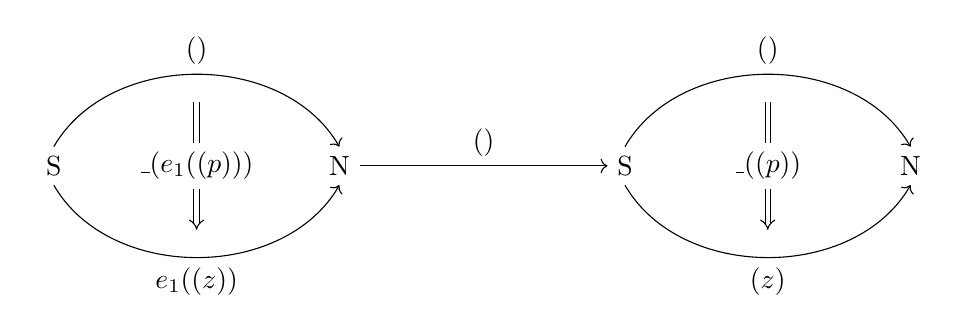
\begin{tikzpicture}
    \matrix (m) [matrix of nodes, column sep=9em] {
      S & N & S & N \\
    };%
    \draw[->] (m-1-1.north) to[bend left=60] node[above, name=Afrom] {$\inv{\mrd(\base)}$} (m-1-2.north);%
    \draw[->] (m-1-1.south) to[bend right=60] node[below, name=Ato] {$\inv{e_1(\mrd(z))}$} (m-1-2.south);%
    \draw[cell] (Afrom) to node[fill=white] {$\inv{\_}(e_1(\mrd(p)))$} (Ato);%
    \draw[->] (m-1-2) to node[above] {$\mrd(\base)$} (m-1-3);%
    \draw[->] (m-1-3.north) to[bend left=60] node[above, name=Bfrom] {$\inv{\mrd(\base)}$} (m-1-4.north);%
    \draw[->] (m-1-3.south) to[bend right=60] node[below, name=Bto] {$\inv{\mrd(z)}$} (m-1-4.south);%
    \draw[cell] (Bfrom) to node[fill=white] {$\inv{\_}(\mrd(p))$} (Bto);%
  \end{tikzpicture}
\end{center}

Taking $p\jdeq{\Sloop}$ gives
$\_\!^{-1}(\mrd(\Sloop)) \cdot_h \refl{n} \cdot_h\  \_\!^{-1}(\mrd(\Sloop^{-1}))$,
which is the special case of the horizontal composition that can be further
simplified to
\begin{align}
  \label{eq:trp-for-e1=e2}
e_{\mrd(\base)}(\_\!^{-1}(\mrd(\Sloop^{-1})) \cdot\_\!^{-1}(\mrd(\Sloop)) = 
e_{\mrd(\base)}(\_\!^{-1}(\refl{\mrd(\base)})).
\end{align}
The latter path is a reflexivity path, so that $\trp{\Sloop}$ is actually homotopic 
to the identity function. Hence we can take for 
$m_f(\Sloop): m_f(\base)=^P_{\Sloop}m_f(\base)$ a simple transport of $\refl{m_f(\base)}$.

For the second statement of the lemma, $(e_0 = e_2)\to\false$,
assume we are given $f(x):R(x)\defeq(e_0(x)=e_2(x))$ for all $x:\Sp$.
We are to prove $\false$. Since the goal is a proposition,
and $N=S$ is connected (as $\pi_1 \Sp$ is contractible),
we can assume $f(N)=n\jdeq\mrd(\base):(N=S)\jdeq R(N)$ and 
$f(S)=s\jdeq\mrd(\base)^{-1}:(S=N)\jdeq R(S)$.
This allows us to reuse parts of the proof of $e_1 = e_2$.
Modulo some transport we have $f(\mrd(z)): n=^R_{\mrd(z)}s$
for all $z:\Sc$. The latter type is equivalent to
$Q(z)\defeq(\mrd(z)^{-1}\cdot n\cdot \mrd(z)^{-1} = s)$.
Thus we get in particular $f'(\mrd(\base)): Q(\base)$ and 
$f'(\mrd(\Sloop)): f'(\mrd(\base))=^Q_{\Sloop}f'(\mrd(\base))$
for some transport $f'$ of $f$.
Transport in the family $Q$ goes like transport in $P$ with $e_1$
replaced by $e_0$, which is $\id$. 
This means that the rhs of Eq.\ref{eq:trp-for-e1=e2} becomes
$p_{02}\defeq e_{\mrd(\base)}(\_\!^{-1}(\mrd(\Sloop\cdot\Sloop)))$.
Transport in $Q$ is equivalent to precompostion with the inverse of $p_{02}$,
and hence $f'(\mrd(\Sloop)): f'(\mrd(\base))=^Q_{\Sloop}f'(\mrd(\base))$
leads to a contradiction if we show
$\mrd(\Sloop\cdot\Sloop) \neq \mrd(\refl{\base})$.
Assume $\mrd(\Sloop\cdot\Sloop) = \mrd(\refl{\base})$.
These are 2-paths of type $\mrd(\base)=\mrd(\base)$.
Since $\hopffam(\mrd{x})(\base) = \iota_1(x)(\base) = x$ for all $x:\Sc$
it follows that $\Sloop\cdot\Sloop = \refl{\base}$ which is absurd. CHECK

The proof of $e_0 = e_3$ is similar to that of $e_1 = e_2$, with some
technical adjustments for the different functions. We leave these to the
reader. We come back to this when we discuss $\Trunc{e_0 = e_3}$.
\end{proof}

\section*{Acknowledgements}
We thank Nicolai Kraus for the insight that
$\mrd(\Sloop\cdot\Sloop) \neq \mrd(\refl{\base})$.

\end{document}

% LocalWords: isomorphisms automorphisms morphisms
 
